\chapter{Architecture et Choix Techniques}
%\minitoc
\clearpage
\label{sec:organisme}

\section{Introduction}
La création d'une distribution Linux personnalisée implique des décisions techniques et conceptuelles précises afin de garantir la sécurité, la stabilité, les performances et le bon fonctionnement du système. Dans ce chapitre, nous détaillerons :

\begin{itemize}
  \item l'architecture générale du système 
  \item les aspects de compilation, d’optimisation et d’automatisation du build.
  \item les choix relatifs au noyau Linux et aux composants essentiels 
  \item la conception et l'architecture du gestionnaire de paquets \textsc{Kraken} ;
  \item la structure du fichier ISO bootable et les mécanismes d’amorçage ;
 


\section{Architecture générale de notre distribution Linux}
Avant de détailler chaque composant, il est essentiel de décrire le cadre général de notre système et de préciser les architectures matérielles que nous visons.
\end{itemize}
\begin{figure}[htbp]
    \centering
    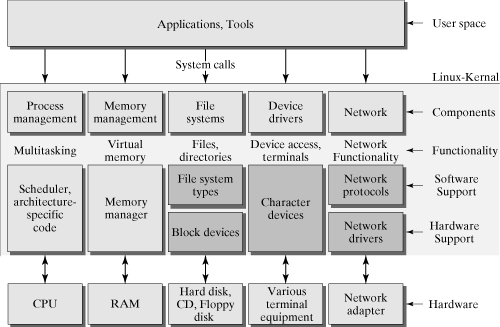
\includegraphics[width=1\textwidth]{images_pfe/linuxarchi.png}
    \caption{Linux System Architecture layers:}
    \label{fig:fhs}
\end{figure}


\label{sec:arch-generale}

\textcolor{red}{TODO: EXPLAIN THIS FIGURE}
\subsection{Architectures cibles}
\label{subsec:arch-cibles}

. Le choix des architectures cibles conditionne en effet les outils de compilation, les optimisations et les bibliothèques à intégrer.

\begin{table}[htbp]
  \centering
  \caption{Types d’architectures de processeur (exemple)}
  \label{tab:architectures}
  \begin{tabular}{|l| l| c| l|}
    \toprule
    \textbf{Architecture} & \textbf{Type} & \textbf{Largeur (bits)} & \textbf{Cas d'utilisation} \\
    \midrule
    x86-64   & CISC & 64           & Stations de travail, serveurs \\
    ARM64    & RISC & 64           & Mobile, embarqué, serveurs    \\
    RISC-V   & RISC & 32/64/128    & Usage académique, matériel sur mesure \\
    POWER    & RISC & 64           & Serveurs d'entreprise, calcul haute performance \\
    \bottomrule
  \end{tabular}
\end{table}

Dans \textsc{Kraken OS}, nous avons choisi comme architectures cibles principales les processeurs AMD/Intel x86\_64 (64 bits), en raison de leur compatibilité étendue et de leur support matériel mature.


\subsection{Normes de \textsc{Kraken OS}}
\label{subsec:standards}

La structure de \textsc{Kraken OS} respecte au maximum les standards Linux suivants :

\begin{itemize}
  \item \textbf{POSIX.1-2008}  ;
  \item \textbf{Filesystem Hierarchy Standard (FHS) v3.0} ;
  \item \textbf{Linux Standard Base (LSB) v5.0 }.
\end{itemize}


\subsubsection{POSIX.1-2008}
\label{sssec:posix}
La norme POSIX (Portable Operating System Interface) définit une interface et un environnement pour systèmes d’exploitation, incluant un interpréteur de commandes (shell) et un ensemble d’utilitaires courants, permettant la portabilité des applications au niveau du code source. Elle s’adresse à la fois aux développeurs d’applications et aux implémenteurs de système.

\paragraph{Pourquoi POSIX est‑il important ?}
\begin{enumerate}
  \item Assurer la \textbf{portabilité} des logiciels entre systèmes de type UNIX (Linux, macOS, BSD, etc.).
  \item Fournir une API cohérente pour les appels système, la gestion des fichiers et le pilotage des processus.
  \item Aider les développeurs à écrire des applications \textbf{cross‑platform} sans réécrire leur code pour chaque OS.
\end{enumerate}


\subsubsection{Filesystem Hierarchy Standard (FHS) v3.0}
\label{sssec:fhs}
Le FHS spécifie les exigences et recommandations de placement des fichiers et répertoires sous systèmes UNIX-like, afin de garantir l’interopérabilité des applications, des outils d’administration, des outils de développement et des scripts, ainsi qu’une documentation uniforme.  



La structure de \textsc{Kraken OS} suit scrupuleusement ce standard (voir figure~\ref{fig:fsl}).

\begin{figure}[H]
  \centering
  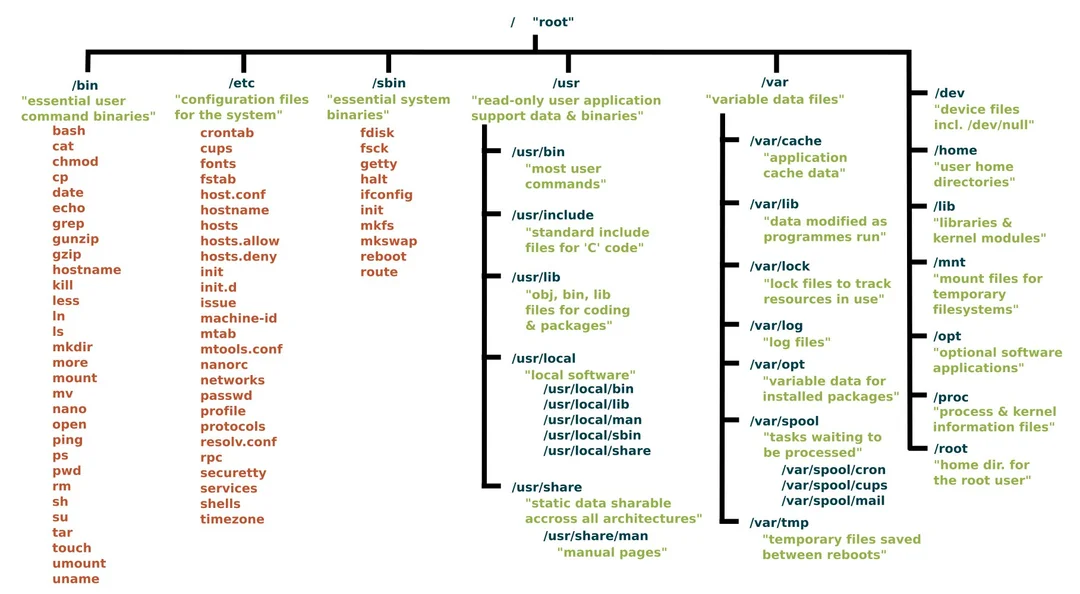
\includegraphics[width=0.85\textwidth]{images_pfe/fslinux.png}
  \caption{Architecture du système de fichiers conforme au standard FHS v3.0}
  \label{fig:fsl}
\end{figure}




Les principaux répertoires comprennent :

\begin{itemize}
    \item \textbf{Répertoires essentiels} :
    \begin{itemize}
        \item \texttt{/bin}, \texttt{/sbin} : Liens symboliques vers \texttt{/usr/bin} et \texttt{/usr/sbin} (conformément aux bonnes pratiques de sécurité)
        \item \texttt{/lib}, \texttt{/lib64} : Liens vers \texttt{/usr/lib} et \texttt{/usr/lib64} (centralisation des bibliothèques)
    \end{itemize}
    
    \item \textbf{Répertoires systèmes critiques} :
    \begin{itemize}
        \item \texttt{/etc} : Configuration système globale (fichiers \texttt{.conf}, scripts d'initialisation)
        \item \texttt{/var} : Données volatiles (logs, bases de données, files d'attente)
        \item \texttt{/proc}, \texttt{/sys} : Interfaces virtuelles pour le monitoring du kernel
    \end{itemize}
    
    \item \textbf{Répertoires fonctionnels} :
    \begin{itemize}
        \item \texttt{/sources} : Isolation des sources logicielles et artefacts de compilation
        \item \texttt{/tools} : Chaîne d'outils temporaire (compilateur croisé, utilitaires bootstrap)
       \item \texttt{/opt} : répertoire dédié aux applications autonomes (monolithiques), comme KDE Frameworks ou Qt6, afin d’éviter les conflits de dépendances qui pourraient survenir lors d’une installation dans un repertoire classique come /usr 

    \end{itemize}
    
    \item \textbf{Répertoires opérationnels} :
    \begin{itemize}
        \item \texttt{/dev} : Représentation hiérarchique des périphériques
        \item \texttt{/mnt}, \texttt{/media} : Points de montage temporaires
        \item \texttt{/srv} : Données spécifiques aux services 
        \item \texttt{/tmp} : Fichiers temporaires (nettoyage automatique via \texttt{tmpfs})
    \end{itemize}
\end{itemize}

Cette architecture répond à trois impératifs fondamentaux :
\begin{enumerate}
    \item Séparation stricte entre composants systèmes et données utilisateur
    \item Isolation des processus de compilation via \texttt{/sources} et \texttt{/tools}
    \item Compatibilité avec les mécanismes kernel (montage automatique de \texttt{/proc}, \texttt{/sys})
\end{enumerate}




\subsubsection{Linux Standard Base (LSB) v5.0}
\label{sssec:lsb}
La Linux Standard Base était un projet collaboratif sous l’égide de la Linux Foundation visant à uniformiser la structure logicielle des distributions Linux. La version 5.0 (2015) se compose de quatre spécifications indépendantes :

\begin{table}[htbp]
  \centering
  \caption{Spécifications de la LSB v5.0}
  \label{tab:lsb-specs}
  \begin{tabular}{|l| p{8cm}|}
    \toprule
    \textbf{Module} & \textbf{Description} \\
    \midrule
    Core     & Interface système de base et utilitaires essentiels \\ \hline
    Desktop  & Composants graphiques et bibliothèques pour environnements de bureau  \\ 
    Languages& Bibliothèques de support pour langages et formats  \\  \hline
    Imaging  & Services d’impression et traitement d’images  \\
    \bottomrule
  \end{tabular}
\end{table}

L’objectif principal de la LSB est de garantir que les logiciels propriétaires peuvent être installés et exécutés sur un système conforme.  
Étant donné que \textsc{Kraken OS} est compilé intégralement à partir des sources, nous vérifions à la compilation que chaque paquet respecte les exigences LSB. Par exemple :

\begin{itemize}
  \item \textbf{Core} : \texttt{bash}, \texttt{coreutils}, \texttt{glibc}, \texttt{binutils}, \texttt{diffutils}, \texttt{grep}, \texttt{gzip}, \texttt{m4}, \dots  
  \item \textbf{Desktop} : \texttt{alsa-lib}, \texttt{atk}, \texttt{cairo}, \texttt{glib2}, \texttt{gdk-pixbuf}, \texttt{gtk+}, \texttt{fontconfig}, \dots  
  \item \textbf{Languages} : \texttt{libxml2}, \texttt{libxslt}, \dots  
  \item \textbf{Imaging} : \texttt{cups}, \texttt{cups-filters}, \texttt{ghostscript}, \texttt{sane-backends}, \dots  
\end{itemize}

\section{Mécanismes fondamentaux et aspects préparatoires pour le chapitre suivant}

À ce stade, nous avons défini qui nous sommes, à quelle famille de systèmes d’exploitation nous appartenons, et précisé notre architecture cible ainsi que les standards à respecter. Nous devons maintenant présenter certains mécanismes et notions clés.

\subsection{Qu’est‑ce qu’un paquet ?}
\label{sssec:definition-paquet}

Un \emph{paquet} est un ensemble de fichiers (bibliothèques, scripts, documentation) fournissant une fonctionnalité précise dans le système : ce paquet peut être un compilateur (\texttt{gcc}), un utilitaire de liens (\texttt{binutils}), un outil de recherche de fichiers (\texttt{findutils}), un utilitaire de base (\texttt{coreutils}), un backend de compilation (\texttt{LLVM}), etc.

Généralement, ce paquet est compressé sous un format tar.gz ,tar.xz,tar.bz2 ou zip, que l’on peut obtenir depuis le site officiel ou en clonant le dépôt GitLab/GitHub.\\
Il contient le code source (outils, scripts, bibliothèques) et un système de build décrivant comment compiler le paquet. Parfois, il inclut aussi les sources de tiers nécessaires à la construction : par exemple, si le programme final est lié dynamiquement à \texttt{libc}, l’auteur du paquet peut inclure une version locale de \texttt{libc} dans ses sources.\\
\textbf{Question :} Les paquets sont-ils liés dynamiquement ? \\
Cette question est cruciale dans un système Linux et nous amène naturellement à distinguer les bibliothèques statiques et les bibliothèques partagées.
\paragraph{Bibliothèques statiques vs partagées}
\begin{enumerate}
  \item \textbf{Bibliothèques statiques} :  
    Les bibliothèques statiques sont des archives de routines (\texttt{libfoo.a}) dont les routines nécessaires sont extraites et liées directement dans l’exécutable.  
  \item \textbf{Bibliothèques partagées (dynamiques)} :  
    Les bibliothèques partagées (\texttt{libfoo.so}) sont chargées une seule fois en mémoire virtuelle, puis partagées par tous les programmes qui les utilisent. Elles sont plus économes en espace.
\end{enumerate}

\begin{figure}[!htbp]
  \centering
  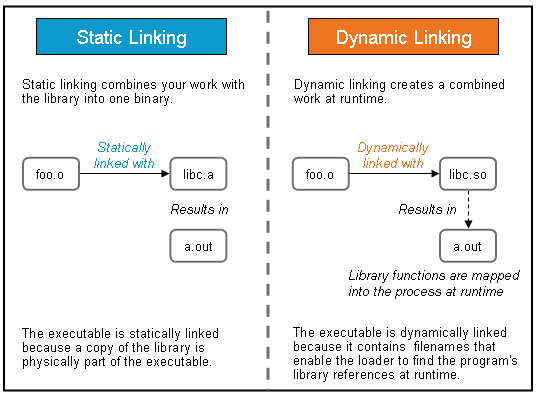
\includegraphics[width=0.85\textwidth]{images_pfe/sharedlibraryvsstatic.png}
  \caption{Bibliothèque statique vs partagée}
  \label{fig:staticsharedl}
\end{figure}

\paragraph{Remarque}  
En général, les mainteneurs développent ces paquets pour une distribution spécifique (Arch, Debian, etc.). Pour les adapter à \textsc{Kraken OS}, il est parfois nécessaire d’appliquer des patches ou de modifier les chemins dans le code source, car l’emplacement des bibliothèques peut varier d’une distribution à l’autre.  
Par exemple, si un paquet s’attend à trouver la bibliothèque \texttt{libX} dans \texttt{/lib} mais que nous l’installons dans \texttt{/usr/lib}, il faudra créer un lien symbolique ou ajuster le chemin de recherche durant le build.





\subsection{Qu’est‑ce que la compilation à partir des sources ?}
\label{subsec:compilation-sources}

Comme mentionné dans le chapitre précédent, nous avons choisi de construire \textsc{Kraken OS} entièrement à partir des sources, pour un contrôle total et une indépendance vis‑à‑vis des distributions généralistes.  
Un système d’exploitation open‑source est le fruit de l’intelligence collective ; chaque ligne de code est accessible et modifiable. L’installation à partir des sources requiert donc de parcourir les sources de chaque paquet et de les compiler soi‑même pour générer les exécutables, la documentation, les bibliothèques, etc.

Généralement, cette étape de compilation s’effectue en utilisant le système de build propre à chaque paquet.

\subsubsection{Qu’est‑ce qu’un système de build ?}
\label{sssec:definition-buildsystem}

Un \emph{système de build} est l’outil ou l’ensemble d’outils orchestrant la configuration, la compilation, le lien et l’installation des sources. Parmi les plus courants :

\begin{table}[h!]
    \centering
    \begin{tabular}{|c|c|p{8cm}|}
        \hline
        \textbf{Logo} & \textbf{Outil} & \textbf{Fonction principale} \\
        \hline
        
\includegraphics[width=0.8cm]{images_pfe/make.png} & Make & Le plus ancien et basique, utilise des Makefiles. \\
        \hline
        
\includegraphics[width=0.8cm]{images_pfe/GNU-Autoconf-768x288.jpg} & Autotools & Traditionnel pour projets open source, gère la compilation croisée. \\
        \hline
        
\includegraphics[width=0.8cm]{images_pfe/zig.png} & Zig & Outil intégré à Zig (compilation C/C++ possible). \\
        \hline
        
\includegraphics[width=0.8cm]{images_pfe/meson_logo.png} & Meson & Alternative moderne et rapide à CMake/Autotools. \\
        \hline
        
\includegraphics[width=0.8cm]{images_pfe/ninja.jpeg} & Ninja & Outil bas niveau, très rapide, utilisé comme backend pour CMake/Meson. \\
        \hline
    \end{tabular}
    \caption{Principaux systèmes de build}
    \label{tab:build_tools_logos}
\end{table}

\subsubsection{Étapes générales de compilation}
\label{sssec:etapes-compilation}

Lors de la construction du système, nous compilons des dizaines de bibliothèques, paquets, etc. Il est donc nécessaire de comprendre comment fonctionne le processus de compilation :

\begin{enumerate}
  \item \textbf{Collecte d’informations}  
    Lire la documentation officielle (wiki, dépôt GitHub/GitLab) pour connaître les dépendances et les options de compilation.\\
    

  \item \textbf{Récupération du code source}  
    Télécharger l’archive (\texttt{.tar.gz}, \texttt{.zip}) à l’aide d’outils tels que \texttt{wget}, \texttt{curl}, ou cloner depuis le dépôt GitLab/GitHub officiel.  
    Vérifier ensuite l’intégrité de l’archive (car le téléchargement peut être interrompu ou corrompu), puis l’extraire et contrôler son contenu (généralement les fichiers du système de build).\\

 \item \textbf{Configuration}  
    À cette étape, le système de build vérifie la présence des bibliothèques, paquets et outils requis, puis active les options souhaitées.  \\
    \textit{Note :} les options de configuration sont très délicates et importantes, car chaque paquet dépend des autres. Il convient donc de se poser deux questions après la configuration de chaque paquet :
    \begin{enumerate}[label=\arabic*)]
      \item Quelle est la configuration nécessaire pour assurer le bon fonctionnement de ce paquet ?
      \item Quelles options doivent être activées maintenant pour que les futurs paquets, qui dépendent de celui-ci, puissent utiliser correctement ses fonctionnalités ?
    \end{enumerate}


    \medskip
    \noindent\textbf{Exemple pratique :}  
    LLVM est un compilateur backend qui gère l’IR (Intermediate Representation). Pour le compiler, il faut construire Clang (runtime LLVM) \textbf{avec le support de}  \texttt{compiler-rt} :

    \begin{verbatim}
cmake \
  -DLLVM_ENABLE_PROJECTS="clang;compiler-rt"
    \end{verbatim}

    \medskip
    \noindent\textbf{a) Exemple de configuration de GCC (Autotools)}  
    \begin{verbatim}
../configure \
  --prefix=/usr \
  --disable-multilib \
  --with-system-zlib \
  --enable-default-pie \
  --enable-default-ssp \
  --enable-host-pie \
  --disable-fixincludes \
  --enable-languages=c,c++,fortran,go,objc,obj-c++,m2
    \end{verbatim}
    \textbf{Explications :}  \\
    \texttt{--prefix} : répertoire d’installation  \\
    \texttt{--disable}/\texttt{--enable} : (dés)activer des fonctionnalités  \\
    \texttt{--with} : préciser un chemin ou une option système \\

    \medskip
    \noindent\textbf{b) Exemple de configuration de LLVM (CMake + Ninja)}  
    \begin{verbatim}
CC=gcc CXX=g++ \
cmake -G Ninja .. \
  -D CMAKE_INSTALL_PREFIX=/usr \
  -D CMAKE_SKIP_INSTALL_RPATH=ON \
  -D LLVM_ENABLE_FFI=ON \
  -D CMAKE_BUILD_TYPE=Release \
  -D LLVM_BUILD_LLVM_DYLIB=ON \
  -D LLVM_LINK_LLVM_DYLIB=ON \
  -D LLVM_ENABLE_RTTI=ON \
  -D LLVM_TARGETS_TO_BUILD="host;AMDGPU" \
  -D LLVM_BINUTILS_INCDIR=/usr/include \
  -D LLVM_INCLUDE_BENCHMARKS=OFF \
  -D CLANG_DEFAULT_PIE_ON_LINUX=ON \
  -D CLANG_CONFIG_FILE_SYSTEM_DIR=/etc/clang
    \end{verbatim}

    \medskip
  
    \noindent\textbf{c) Exemple de configuration de GLib (Meson)}  
    \begin{verbatim}
meson setup builddir \
  --prefix=/usr \
  --buildtype=release \
  -D introspection=disabled \
  -D man=true
    \end{verbatim}
    \textbf{Explications :}  \\
    \texttt{--buildtype} : mode de compilation (debug/release)\\

  \item \textbf{Compilation}  
    Après configuration, nous lancer la construction des binaires via le système de build :
    \begin{verbatim}

 make ou ninja
    \end{verbatim}

  \item \textbf{Tests}  
    Après compilation, nous tester le paquet, surtout s’il est critique :
    \begin{verbatim}
make check ou ninja test
    \end{verbatim}

  \item \textbf{Installation}  
   c.a.d installer les fichiers dans l’arborescence cible :
    \begin{verbatim}
make install ou ninja install
    \end{verbatim}

  \item \textbf{Post‑configuration}  
     Adapter les fichiers de configuration et installer la documentation.

  \item \textbf{Nettoyage et validation}  
    Supprimer les fichiers temporaires et le répertoire de build, tout en conservant l’archive source pour d’éventuelles recompilations.
\end{enumerate}
\clearpage
\subsection{Qu’est‑ce que le \emph{bootstrap} ?}
\label{subsec:bootstrap}
\begin{figure}[H]
  \centering
  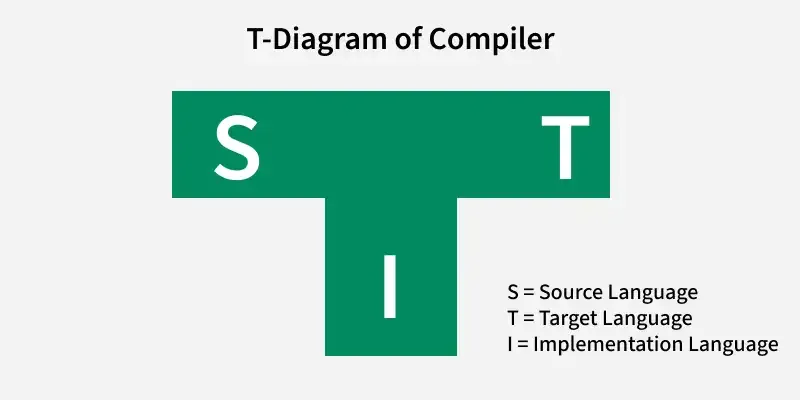
\includegraphics[width=0.85\textwidth]{images_pfe/bootstrap.png}
  \caption{Schéma de l’amorçage d’un compilateur}
  \label{fig:bootstrap}
\end{figure}

Lors de la compilation de paquets à partir des sources, nous rencontrons souvent des problèmes liés à l’amorçage (\emph{bootstrap}).  
Le \emph{bootstrap} (ou amorçage) permet de compiler un composant dont le compilateur est écrit dans le même langage — et donc non disponible a priori sur la machine de construction. (java , go, rust...)

\bigskip
\noindent
\textbf{Problème}  
Supposons que l’on veuille construire le langage \texttt{Go}, dont le compilateur est écrit en \texttt{Go} lui‑même. Comment produire un exécutable quand aucun compilateur \texttt{Go} n’est encore installé ?

\medskip
\noindent
\textbf{Solution}  
On utilise un \emph{bootstrap} : un binaire pré‑compilé ou un compilateur antérieur sert à générer la première version du compilateur \texttt{Go}. Ce compilateur issu du bootstrap est ensuite utilisé pour compiler la version finale.  
Vous pouvez simplement comprendre ce concept comme « compiler un compilateur à l’aide d’un compilateur préexistant pour générer le compilateur définitif ! »



Cette méthode générale s’applique à tout langage ou outil dont le compilateur est en auto‑hospitage (\emph{self‑hosting}). Elle garantit l’isolement complet et la traçabilité de chaque étape de construction.


%-------------------compiler ------------------
\subsection{Compilateur croisé}
\label{subsec:cross-compiler}

La compilation croisée est utilisée pour construire un compilateur et sa chaîne d’outils pour une machine différente de celle servant à la compilation.  
Simplement pour générer des exécutables qui fonctionneront sur une machine différente de la machine hôte : par exemple, on peut utiliser un cross-compiler installé sur une architecture x86\_64 pour produire des exécutables destinés à l’architecture ARM .

\begin{figure}[!htbp]
  \centering
  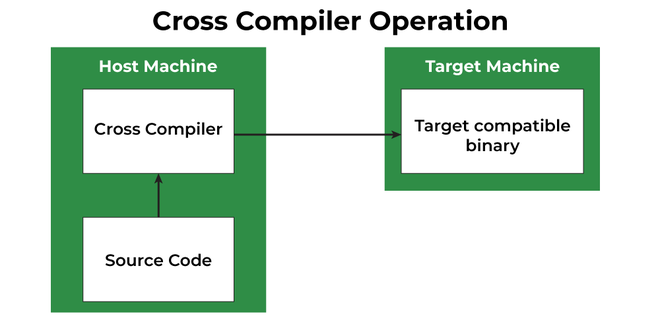
\includegraphics[width=0.85\textwidth]{images_pfe/crosscompiler.png}
  \caption{Compilateur croisé}
  \label{fig:crosscompiler}
\end{figure}

\subsubsection{Notions clés}
\begin{itemize}
  \item \textbf{Build} : machine utilisée pour la compilation.
  \item \textbf{Host} : machine sur laquelle les programmes compilés seront exécutés.
  \item \textbf{Target} : architecture cible pour laquelle le code est généré.
\end{itemize}


\subsubsection{Exemple pratique : Canadian Cross}
La méthode dite « Canadian Cross » se déroule en trois étapes successives, impliquant trois machines distinctes.

Nous disposons d'un compilateur natif sur une machine lente (machine A), appelé \texttt{ccA}. Nous disposons également d'une machine rapide (machine B) sans compilateur, et nous souhaitons produire du code pour une troisième machine lente (machine C). Nous allons construire un compilateur pour la machine C en trois étapes :

\begin{table}[!htbp]
  \centering
  \caption{Processus de compilation « Canadian Cross »}
  \label{tab:canadian-cross}
  \begin{tabular}{|l|l|l|l|p{6cm}|}
    \hline
    \textbf{Étape} & \textbf{Build}    & \textbf{Host}    & \textbf{Target}  & \textbf{Action}                                      \\
    \hline
    1              & A (lente)         & A                & B                & Compilation de \texttt{cc1}  avec \texttt{ccA} sur A    \\
    \hline
    2              & A                 & B                & C                & Compilation de \texttt{cc2} à l’aide de \texttt{cc1} sur A                \\
    \hline
    3              & B (rapide)        & C                & C                & Compilation de \texttt{ccC} (natif) avec \texttt{cc2} sur B                \\
    \hline
    4              & C                 & C                & C                & Rebuild et test de \texttt{ccC} avec lui‑même sur C                      \\
    \hline
  \end{tabular}
\end{table}

Dans cet exemple :
\begin{itemize}
  \item \textbf{cc1}, \textbf{cc2} : compilateurs croisés, générant du code pour une autre architecture.
  \item \textbf{ccA}, \textbf{ccC} : compilateurs natifs, générant du code pour leur machine hôte.
\end{itemize}

\bigskip
\noindent
\textbf{Remarque :} dans le cas de \textsc{Kraken OS}, la machine hôte et la machine cible sont identiques (même architecture).  
Pourquoi utiliser alors un compilateur croisé ?  
Tout simplement pour l’isolation : la cross‑compilation présente un grand avantage : tout ce qui est compilé en croisé ne peut pas dépendre de l’environnement hôte.  

\medskip
\noindent
\textbf{Solution :}  
Nous mettrons en œuvre un « faux » cross‑compiler. Cette approche sera détaillée dans le chapitre suivant.

%kernel ---------------------------------------

\subsection{Noyau et choix des modules}
\label{subsec:noyau-modules}

Le noyau Linux est l’élément central d’un système d’exploitation, responsable de la gestion des ressources matérielles et de l’interaction avec le matériel. Le projet Linux est l’un des plus importants projets open-source au monde, rassemblant des milliers de contributeurs et générant des millions de lignes de code modifiées à chaque version. \\ 
Le mainteneur principal : Linus Torvalds.


Avant de configurer et compiler le noyau, il est essentiel de comprendre ses composants fondamentaux (voir figure~\ref{fig:kernel-arch}) :

\begin{figure}[H]
  \centering
  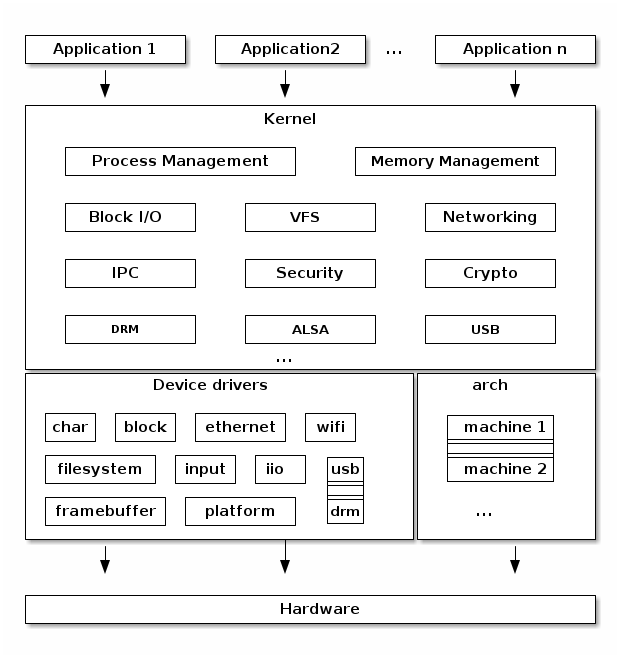
\includegraphics[width=0.85\textwidth]{images_pfe/kernelarchitecture.png}
  \caption{Architecture générale du noyau Linux}
  \label{fig:kernel-arch}
\end{figure}

\begin{description}
  \item[1. Architecture (\texttt{arch})]  
    Contient le code spécifique aux architectures matérielles (x86, ARM, MIPS, PowerPC, IBM S/390, etc.), parfois subdivisé en code machine spécifique.
  \item[2. Pilotes de périphériques (Device Drivers)]  
    Mise en œuvre d’un modèle unifié pour gérer les périphériques : détection, état, bus d’attache et liaison avec le pilote approprié.
  \item[3. Gestion des processus (Process Management)]  
    Création, ordonnancement et terminaison des processus. Implémentation des appels \texttt{fork()}, \texttt{exec()}, \texttt{wait()} et des threads POSIX via la structure \texttt{task\_struct}.
  \item[4. Gestion de la mémoire (Memory Management)]  
    Allocation et libération de la mémoire physique et virtuelle : pagination, swap, \texttt{mmap()}, \texttt{brk()}, allocateurs SLAB et \texttt{vmalloc}.
  \item[5. Gestion du Block I/O (Block I/O Management)]  
    Création et ordonnancement des requêtes d’E/S sur périphériques bloc : RAID logiciel, LVM, fusion et tri des requêtes, planification par ordonnanceurs d’I/O.
\end{description}

%\begin{figure}[H]
%  \centering
 % 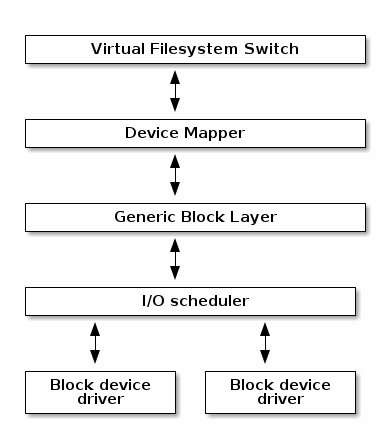
\includegraphics[width=0.85\textwidth]{images_pfe/iomanagmemnt.png}
%  \caption{Architecture du sous‑système Block I/O}
%  \label{fig:io-management}
%\end{figure}
\subsubsection{Configuration du noyau}

Dans le noyau Linux, il existe deux types de configurations principales :

\begin{enumerate}
  \item \textbf{Intégrée au noyau (built-in)}

  Lorsqu'une option est activée en tant qu’élément intégré (\texttt{built-in}), cela signifie qu’elle est compilée directement dans l’image binaire du noyau (\texttt{vmlinuz}).

  \textbf{Caractéristiques :}
  \begin{itemize}
    \item \textbf{Toujours disponible} : Pas besoin de la charger manuellement, elle fait partie du noyau dès le démarrage.
    \item \textbf{Pas de surcharge à l’exécution} : Exécution plus rapide, car le code est déjà en mémoire.
    \item \textbf{Taille du noyau plus grande} : Augmente le temps de démarrage et l’utilisation de la mémoire.
    \item \textbf{Critique pour le démarrage} : Les pilotes matériels essentiels (ex. : contrôleurs de disque, systèmes de fichiers) doivent être intégrés si nécessaires pendant les premières étapes du démarrage (avant le chargement de l’espace utilisateur ou de l’initramfs).
  \end{itemize}

  \item \textbf{Modules chargeables (Loadable Kernel Modules)}

  Les fonctionnalités marquées comme \texttt{m} (module) sont compilées séparément sous forme de fichiers objets \texttt{.ko} (Kernel Object), stockés dans \texttt{/lib/modules}.

  \textbf{Caractéristiques :}
  \begin{itemize}
    \item \textbf{Chargés à la demande} : Manuellement via \texttt{modprobe}, ou automatiquement via \texttt{udev}.
    \item \textbf{Utilisation mémoire réduite} : Les modules ne sont chargés que lorsqu’ils sont nécessaires.
    \item \textbf{Flexibilité de mise à jour} : Les modules peuvent être recompilés ou rechargés sans nécessiter de redémarrage du système.
  \end{itemize}
\end{enumerate}




Pour \textsc{Kraken OS}, nous avons retenu le noyau Linux \texttt{6.10.5}, garantissant un équilibre entre stabilité et fonctionnalités récentes. Nous avons activé uniquement les modules nécessaires aux architecture cible  x86\_64, et désactivé les options optionnelles afin de réduire l’empreinte mémoire et d’optimiser les performances. Les détails précis de ces configurations seront présentés dans le chapitre suivant.

\bigskip
L’un des aspects les plus enthousiasmants d’un système d’exploitation moderne — protection, concurrence, virtualisation, allocation de ressources et stockage fiable — est qu’ils se retrouvent aujourd’hui dans de nombreux domaines de l’informatique, au‑delà des seuls noyaux. Il est impossible de concevoir des systèmes informatiques résilients, sécurisés et flexibles sans appliquer ces concepts fondamentaux.

\subsection{Systèmes d'initialisation : System V}

\subsubsection{System V}

System V est le processus de démarrage classique utilisé dans les systèmes Unix et dérivés, comme Linux, depuis environ 1983. Il repose sur un petit programme appelé \texttt{init}, dont le rôle est de configurer les processus de base du système, comme le service de connexion (via \texttt{getty}), et d’exécuter un script principal, souvent nommé \texttt{rc}. Ce dernier orchestre une série de scripts additionnels permettant d'initialiser les différents services et composants du système.

Le comportement du programme \texttt{init} est contrôlé par le fichier \texttt{/etc/inittab}, qui organise l'initialisation autour de différents niveaux d'exécution (runlevels). Dans \textbf{KRAKEN OS}, ces niveaux sont utilisés comme suit :

\begin{itemize}
  \item \textbf{0} — arrêt du système (halt)
  \item \textbf{1} — mode mono-utilisateur (Single user mode)
  \item \textbf{2} — niveau définissable par l'utilisateur
  \item \textbf{3} — mode multi-utilisateur complet (sans interface graphique)
  \item \textbf{4} — niveau définissable par l'utilisateur
  \item \textbf{5} — mode multi-utilisateur complet avec gestionnaire d'affichage
  \item \textbf{6} — redémarrage du système (reboot)
\end{itemize}

Le niveau d'exécution par défaut dans KRAKEN est généralement le niveau 3 ou 5, selon que l'on souhaite démarrer avec ou sans interface graphique.

\paragraph{Avantages}

\begin{itemize}
  \item Système établi et bien documenté.
  \item Facile à personnaliser via des scripts shell.
\end{itemize}

\paragraph{Inconvénients}

\begin{itemize}
  \item Temps de démarrage plus long : un système KRAKEN de base démarre en 8 à 12 secondes, mesuré depuis le premier message du noyau jusqu'à l'invite de connexion. La connectivité réseau est généralement établie 2 secondes après l'invite.
  \item Traitement séquentiel des services au démarrage : un retard dans un processus, comme la vérification du système de fichiers, retarde tout le démarrage.
  \item Absence de support natif pour les fonctionnalités modernes comme les groupes de contrôle (cgroups) et le partage équitable des ressources entre utilisateurs.
  \item Ajout de nouveaux scripts nécessite une planification manuelle et une séquence d'exécution statique.
\end{itemize}

\subsection{Qu'est-ce qu'un bootloader ?}
Cette étape critique nécessite une attention particulière sous peine de rendre le système inopérant.\\
Il existe deux grands chargeurs d'amorçage (bootloaders) pour les systèmes Unix : \textbf{GRUB} et \textbf{Syslinux}.  
Dans \textsc{Kraken OS}, nous avons choisi d’utiliser \textbf{GRUB} pour démarrer le système depuis le disque, et \textbf{Syslinux} pour l’intégration dans le fichier ISO bootable.  

Nous parlerons de \textbf{Syslinux} dans les chapitres suivants, mais concentrons-nous maintenant sur \textbf{GRUB}.

GRUB signifie \textit{GRand Unified Bootloader}, conçu à l’origine par Erich Stefan Boleyn.

\medskip
\noindent
En bref, un \textit{bootloader} est le premier programme logiciel exécuté au démarrage d’un ordinateur. Il est responsable du chargement et du transfert de contrôle vers le noyau du système d’exploitation.  
Ce dernier se charge ensuite de l’initialisation complète du système.

Pour visualiser ce processus, reportez-vous à la figure suivante qui montre un schéma simplifié du démarrage :

\begin{figure}[H]
  \centering
  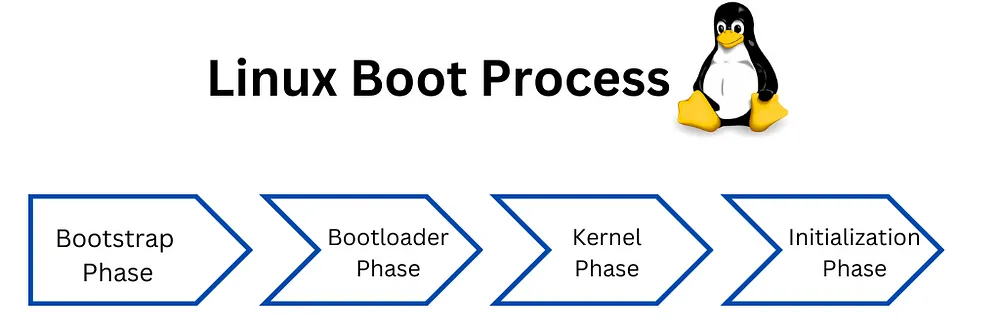
\includegraphics[width=0.85\textwidth]{images_pfe/simplebootprocess.png}
  \caption{Processus de démarrage simplifié}
  \label{fig:botprocess}
\end{figure}

Nous discuterons ce processus plus en détail dans le chapitre sur la création de l’ISO.

\bigskip
\noindent
GRUB utilise une nomenclature spécifique pour référencer les disques et partitions.  
La syntaxe est de la forme \texttt{(hdn,m)} où :
\begin{itemize}
  \item \texttt{n} est le numéro du disque dur (en commençant à 0)
  \item \texttt{m} est le numéro de la partition (en commençant à 1 dans GRUB 2)
\end{itemize}

\noindent
Par exemple :

\begin{table}[h!]
    \centering
    \begin{tabular}{|l|l|}
    \hline
    \textbf{Disque physique} & \textbf{Notation GRUB} \\
    \hline
    \texttt{/dev/sda1} & \texttt{(hd0,1)} \\
    \texttt{/dev/sdb3} & \texttt{(hd1,3)} \\
    \hline
    \end{tabular}
    \caption{Correspondance des partitions selon GRUB}
    \label{tab:grub-part}
\end{table}


\clearpage
\section{Le gestionnaire de paquets \textsc{Kraken}}
\label{sec:kraken-pkg}

Un gestionnaire de paquets est un outil  permettant d’automatiser les processus d’installation, de mise à jour et de suppression de paquets sur un système Linux. 

Malheureusement, le mécanisme de gestion des paquets n’est pas un aspect purement théorique. En pratique, chaque grande distribution conçoit son propre gestionnaire de paquets, selon une philosophie qui lui est propre.\\
À ce stade, il est donc important de comprendre que nous devons inventer un nouveau gestionnaire de paquets conçu et développé entièrement à partir de zéro, sans s’appuyer sur
un autre gestionnaire existant

L’objectif du gestionnaire de paquets \textsc{Kraken} est de fournir une solution à la fois simple et efficace pour l’installation, la mise à jour, la configuration et la suppression des logiciels. Il prend en charge les dépendances, la gestion des versions, ainsi que toutes les tâches complexes afin de faciliter la gestion des programmes.



%\subsection{Fonctionnalités du gestionnaire de paquets sous Linux}
%\label{subsec:kraken-fonctions}

%\begin{itemize}
 % \item \textbf{Installation}  
  %  Permet d’installer des paquets depuis des dépôts distants . Gère automatiquement les dépendances
  %\item \textbf{Résolution de dépendances}  
  %  Analyse les besoins de chaque paquet et récupère automatiquement les paquets requis.
  %\item \textbf{Mise à jour (upgrade)}  
  %  Met à jour les paquets installés vers leurs dernières versions, assurant ainsi la sécurité et la fraîcheur du système.
  %\item \textbf{Suppression}  
  %  Désinstalle les paquets et leurs dépendances obsolètes, sans laisser de fichiers orphelins.
  %\item \textbf{Interrogation (query)}  
  %  Fournit des commandes pour lister les paquets installés, les mises à jour disponibles et les détails de %chaque paquet.
%\end{itemize}



\subsection{kraken architecture }


 


\begin{figure}[H]
  \centering
  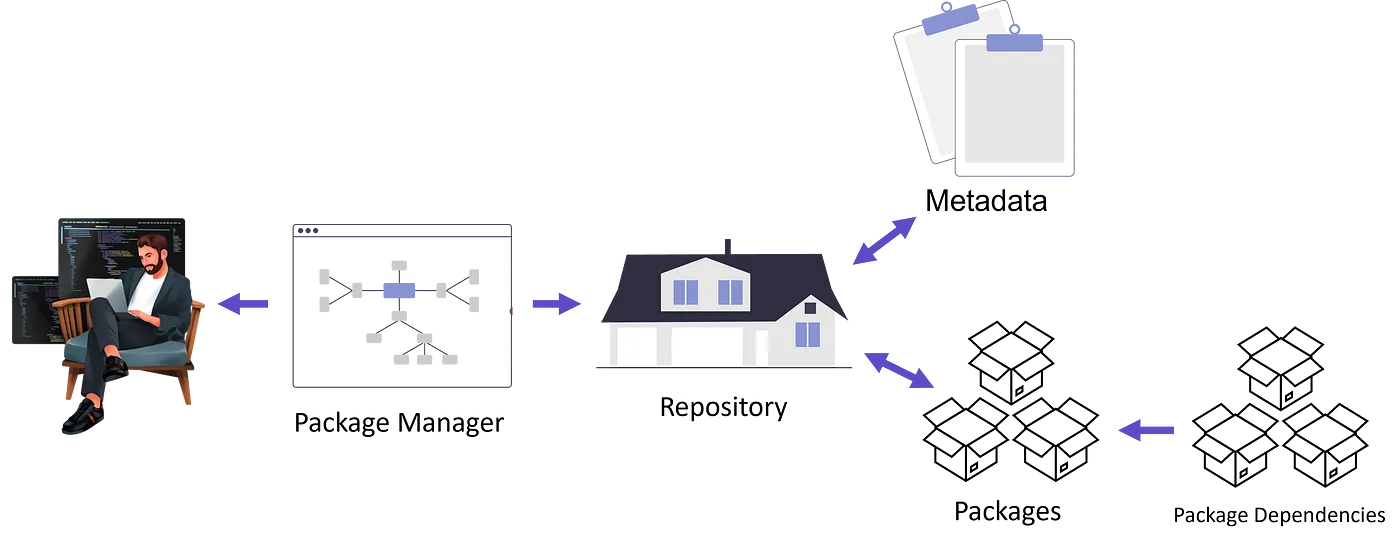
\includegraphics[width=0.85\textwidth]{images_pfe/packagemanager.png}
  \caption{krakne package manager architecture }
  \label{fig:packagemanager}
\end{figure}


 Cette figure illustre la manière dont nous avons conçu notre gestionnaire de paquets. 
 Le premier composant de Kraken est le \textbf{dépôt} , où sont stockées les métadonnées des paquets. Chaque paquet est décrit par un fichier \textbf{pkgbuild.kraken}, qui définit la procédure d'installation du paquet sur Kraken OS à l'aide du gestionnaire de paquets Kraken. 
 Le deuxième composant correspond aux outils du gestionnaire de paquets, qui permettent de récupérer, interroger et installer les paquets depuis le dépôt vers le système. 

Avant de commencer à développer le gestionnaire de paquets \textsc{Kraken}, il est essentiel de comprendre un problème majeur connu sous le nom de \textbf{« dependency hell »} (l’enfer des dépendances).

\subsection{Qu’est‑ce qu’une dépendance de paquet ?}
\label{subsec:dependency}

Une dépendance de paquet est l’ensemble des autres paquets, bibliothèques ou outils requis pour qu’un paquet puisse s’installer et fonctionner correctement. Pour installer un paquet, il faut résoudre automatiquement toutes ses dépendances dans le bon ordre. 

On peut visualiser ce processus comme un graphe orienté : chaque nœud représente un paquet, et chaque arc pointe vers un paquet dont il dépend.  

\begin{figure}[H]
  \centering
  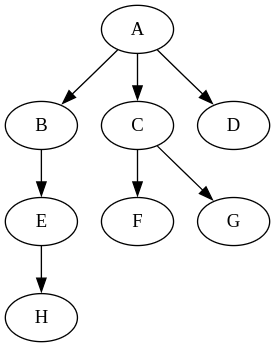
\includegraphics[width=0.5\textwidth , height=10cm]{images_pfe/genralgraphexemple.png}
  \caption{Exemple de graphe de dépendances}
  \label{fig:exempledepndencygraph}
\end{figure}


Pour installer le paquet \texttt{A} :
\begin{enumerate}
  \item Il faut d’abord installer \texttt{B}, \texttt{C} et \texttt{D}.
  \item Pour \texttt{B}, on doit installer \texttt{E}, lui‑même dépendant de \texttt{H}.
  \item Une fois \texttt{B}  installés, on revient au sous‑graphe de \texttt{C} et on installe \texttt{F} et \texttt{G}.
\end{enumerate}

Cette résolution suit en général un algorithme de \emph{parcours en profondeur} (DFS) du graphe de dépendances.  

Cependant, dans la pratique, le graphe peut être très vaste (des dizainess de paquets) et contenir  des cycle. Il faut alors mettre en place des stratégies d’optimisation (caching, détection de cycles, etc.). Tous ces enjeux sont regroupés sous le terme \textbf{« enfer des dépendances »} (Dependency Hell).


\subsection{Premier problème : dépendances circulaires}
\label{subsec:circular-dependencies}

Une dépendance circulaire survient lorsqu’un paquet A dépend d’un paquet B, qui lui-même dépend de A. Cette situation bloque la résolution automatique des dépendances, car ni A ni B ne peut être installé en premier sans l’autre.

\begin{figure}[H]
  \centering
  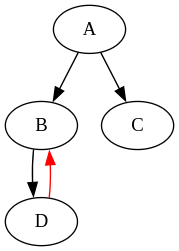
\includegraphics[width=0.3\textwidth, height=8cm]{images_pfe/CERCULARDEP.png}
  \caption{Exemple simple de dépendance circulaire}
  \label{fig:circular-dep}
\end{figure}



Sur la figure~\ref{fig:circular-dep}, pour installer \texttt{B}, il faut d’abord installer \texttt{D}, qui dépend de \texttt{B}, bouclant ainsi le processus.

\paragraph{Cas d’usage réel : outils multimédia}
Considérons deux paquets :
\begin{itemize}
  \item \textbf{DocumentConverter} : convertit des documents (PDF → Word, etc.) et nécessite \texttt{FileViewer} pour prévisualiser les fichiers convertis.
  \item \textbf{FileViewer} : affiche des documents (PDF, Word, ODT, etc.) et nécessite \texttt{DocumentConverter} pour convertir les formats non pris en charge.
\end{itemize}

\begin{figure}[H]
  \centering
  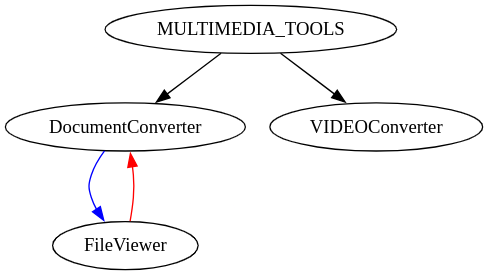
\includegraphics[width=0.5\textwidth]{images_pfe/depcycleexemple.png}
  \caption{Boucle de dépendance entre \texttt{DocumentConverter} et \texttt{FileViewer}}
  \label{fig:depcycle-multimedia}
\end{figure}



\subsubsection*{Stratégie de résolution}
Pour casser la boucle de dépendances, on procède en plusieurs étapes :
\begin{enumerate}
  \item \textbf{Installation initiale de FileViewer minimal}  
    Compiler et installer \texttt{FileViewer} sans le support de conversion.
  \item \textbf{Installation de DocumentConverter}  
    Compiler et installer \texttt{DocumentConverter}, qui s’appuie sur le FileViewer minimal.
  \item \textbf{Recompilation de FileViewer}  
    Recompiler \texttt{FileViewer} en activant le support de \texttt{DocumentConverter}.
  \item \textbf{Installation finale de FileViewer complet}  
    Installer la nouvelle version de \texttt{FileViewer} avec toutes les fonctionnalités.
\end{enumerate}

Cette méthode garantit que chaque paquet et ses dépendances sont disponibles au moment opportun, évitant ainsi l’« enfer des dépendances » engendré par les boucles circulaires. 



\subsection{Deuxième problème : conflit de dépendances}
\label{subsec:dependency-conflict}

Un conflit de dépendances survient lorsque deux paquets, ou plus, requièrent la même bibliothèque ou le même composant, mais chacun spécifie une version différente. Par exemple, sur la figure~\ref{fig:dependency-conflict} :

\begin{figure}[H]
  \centering
  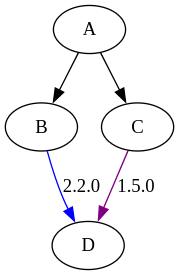
\includegraphics[width=0.3\textwidth, height=5cm]{images_pfe/dpendencyconfligt.png}
  \caption{Exemple de conflit de dépendances }
  \label{fig:dependency-conflict}
\end{figure}

Ici, \texttt{B} dépend de \texttt{D} en version 2.2.0, alors que \texttt{C} exige la version 1.5.0. Le gestionnaire doit alors choisir :

\begin{itemize}
  \item Installer la version la plus récente (2.2.0), au risque de casser \texttt{C}.
  \item Installer la version la plus ancienne (1.5.0), au risque de manquer des correctifs ou fonctionnalités pour \texttt{B}.
  \item Installer simultanément les deux versions, .  au risque de conflit dans le systeme
\end{itemize}

\subsubsection*{Stratégies de résolution}

Malheureusement, ce problème est, selon moi, un problème non résolu en informatique. J'ai effectué de nombreuses recherches pour tenter de trouver une solution, mais chaque gestionnaire de paquets essaie seulement de le contourner sans réellement parvenir à une solution pratique. En général, ils se contentent d'afficher un message à l'utilisateur pour l'informer qu’un conflit existe entre deux ou plusieurs paquets. C’est également l’approche que nous avons choisie. Par exemple, le gestionnaire de paquets \texttt{pacman} ou encore \texttt{xbps} de Void Linux adoptent cette stratégie.




\subsection{Pourquoi avons-nous besoin d’un mécanisme de suivi des métadonnées des paquets ?}
\label{subsec:suivi-fichiers}

Dans un système Linux, l’installation d’un paquet répartit ses fichiers sur de nombreux emplacements :
\begin{itemize}
  \item Binaires : \texttt{/usr/bin}, \texttt{/usr/local/bin}, etc.  
  \item Bibliothèques : \texttt{/lib}, \texttt{/usr/lib}, \texttt{/lib64}, etc.  
  \item En-têtes : \texttt{/usr/include}, etc.  
  \item Fichiers de configuration : \texttt{/etc}.  
  \item Documentation : \texttt{/usr/share/doc}, \texttt{/usr/share/man}, etc.  
  \item Éléments supplémentaires : \texttt{/opt}, \texttt{/var}, etc.  
\end{itemize}

Sans mécanisme de suivi, désinstaller proprement un paquet devient fastidieux : il faudrait rechercher manuellement chacun de ses fichiers dans tout le système, ce qui est impraticable quand on gère des centaines de milliers de fichiers.

\textbf{Notre solution :} développer un mécanisme de « fausse installation ». Ce mécanisme doit générer des fichiers de métadonnées contenant tous les chemins des fichiers et répertoires créés ou modifiés lors de l’installation du paquet. Nous détaillerons cette approche dans le chapitre suivant dédié au développement et à l’implémentation.





\clearpage
\section{Architecture de l’ISO bootable}

Après avoir terminé la construction du système, nous devons fournir à l’utilisateur une image ISO bootable, qu’il pourra installer sur sa machine locale, que ce soit dans une machine virtuelle ou directement sur un matériel physique.

Le processus de génération de l’image ISO est aussi complexe que la construction du système elle-même. Il est donc nécessaire de bien comprendre le processus de démarrage.

\begin{figure}[H]
  \centering
  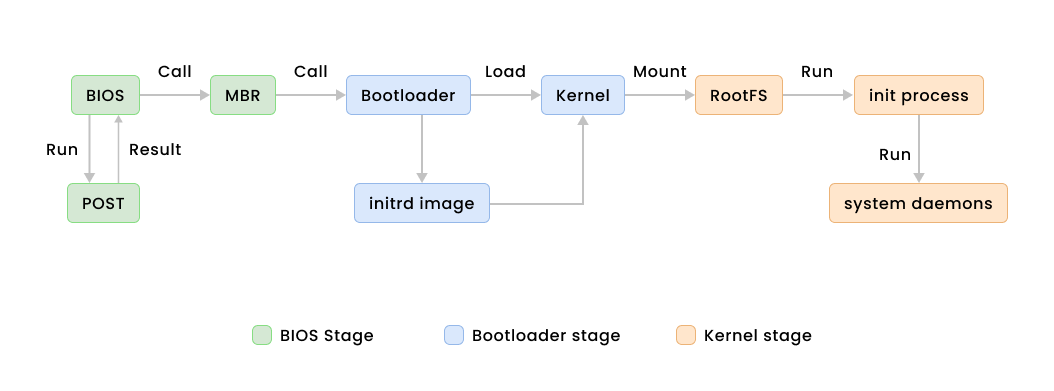
\includegraphics[width=1\textwidth, height=10cm]{images_pfe/bootloader process.png}
  \caption{Processus de démarrage de Kraken OS}
  \label{fig:kbootproc}
\end{figure}



Nous avons décidé que l’ISO bootable de Kraken contiendra :

\begin{enumerate}
  \item \textbf{Un bootloader (chargeur d’amorçage)} — Nous avons choisi \texttt{syslinux}. Il s’agit du premier programme chargé en mémoire au démarrage de l’ordinateur. Il localise le noyau du système d’exploitation choisi et le charge en mémoire. Il gère également le disque RAM initial (\texttt{initrd}).
  
  \item \textbf{L’image \texttt{initrd}} — Elle fournit un ensemble minimal d’outils, de pilotes et d’utilitaires nécessaires pour monter le système de fichiers racine. Elle contient les pilotes essentiels pour les contrôleurs de stockage, les systèmes de fichiers, et les autres composants matériels requis par le noyau pour accéder au vrai système de fichiers racine.
  
  \item \textbf{Le système de fichiers \texttt{rootfs}} — Nous devons empaqueter notre système Kraken OS, le mapper depuis un disque virtuel, puis le compresser dans un fichier \texttt{rootfs}. Ce système de fichiers racine est le point de départ de toute la hiérarchie du système de fichiers. Il est monté par le noyau lors du processus de démarrage, et tous les autres systèmes de fichiers sont montés comme sous-répertoires.
  
  \item \textbf{Une application graphique et un script Bash} — Ces deux outils géreront l’installation du système Kraken OS depuis l’environnement live de l’ISO vers le disque souhaité par l’utilisateur.
\end{enumerate}







\section{Conclusion}
Dans ce chapitre nous avons détaillé les choix techniques et l'architecture de projet. Nous avons vu la sélection de noyau et les modules, les stratégies d'optimisation des, ainsi que les mesures de mesures de sécurité déployés. Enfin, nous avons présenté le gestionnaire de paquets Kraken et les outils intégré à la distributions.

Dans le chapitre suivant, nous nous aborderons le processus de développement et d'implémentations, en détaillant les étapes de construction et les tests effectués sur la distribution.

\medskip



